\documentclass[12pt]{scrartcl}
\usepackage[a4paper,bindingoffset=0.2in,%
left=0.5in,right=0.5in,top=1in,bottom=1in,%
footskip=.25in]{geometry}
\usepackage[affil-it]{authblk}
\usepackage[utf8]{inputenc}
\usepackage{listings}
\usepackage{color}
\usepackage{xcolor}
\usepackage{pdfpages}
\usepackage{graphicx}
\usepackage{textcomp}
\usepackage{hyperref}
\usepackage{dirtree}
\usepackage{footnotebackref}

\definecolor{codegreen}{rgb}{0,0.6,0}
\definecolor{codegray}{rgb}{0.5,0.5,0.5}
\definecolor{codepurple}{rgb}{0.58,0,0.82}
\definecolor{backcolour}{rgb}{1.0,1.0,1.0}

\newcommand{\folder}[2]{}


\lstdefinestyle{mystyle}{
	backgroundcolor=\color{backcolour},   
	commentstyle=\color{codegreen},
	keywordstyle=\color{magenta},
	numberstyle=\tiny\color{codegray},
	stringstyle=\color{codepurple},
	basicstyle=\scriptsize,
	breakatwhitespace=false,         
	breaklines=true,                 
	captionpos=b,                    
	keepspaces=true
}


\lstset{style=mystyle}
\begin{document}
	\title{%
		Mercantile Ships
	}
	\author{Aly Shmahell\\%
		\href{aly.shmahell@gmail.com}{aly.shmahell@gmail.com}
	}
	\affil{%
		3rd Year Student\\
		Department of Computer Science, University of L'Aquila\\
		Databases - Lab Module\\
		Prof. Pierluigi Pierini
		}
	\date{Jan 9th 2018}
	
	\maketitle	
	\newpage
	\begin{center}
		\section*{\hfil \hfil  Abstract \hfil }
	\end{center}
		In this document I will showcase the 3 stages of design of the "Mercantile Ships" Database.\\
		In this effort, and under permission from the requirements file, I made some decisions regarding the techniques and tools used in the design process.\\
		In some extreme cases I had to settle for less than optimal solution either for conformity purposes (the solution conforms best to the design stage) or for practicality, or for highlighting the optimal solution.\\
\newpage
\section*{\textbf{Design and Tool Choices}}
Having Ubuntu linux as my main operating system, I had a small set of tools to choose from, the obvious ones anyways.\\
For the Conceptual Schema Dia was the most suggested on general forums, but it is highly outdated and full of bugs (as tested on my system), also, but it didn't offer any integrated features.\\

This is why I chose \textbf{MySQL Workbench}, it comes the most recommended from DB professionals, doesn't offer ER design capability, but better, it comes equipped with an EER designer, it offers backward engineering, forward engineering, SQL scripting, python scripting, SQL database connection, and with its SQL linter/debugger, the three stages of the DB design get improved live and professionally.\\

One note on MySQL Workbench, on its default settings, it only cares about relationships that translate into Foreign Keys, all other operations can be added as SQL routines(procedures)/triggers/scripts. Which makes sense, because this is how we actually translate from Conceptual Design to Logical Design.\\
But, the EER model in MySQL Workbench can be tweaked a little if someone wants to to add non-key-type relations. However, I chose to stick with the defaults.\\

There are some other tools which I found (rather late), like draw.io, it's just a modeling tool, much like Dia, but it is more up to date and it has some nice features like adding your own shape (you have to script it in xml) so you can represent any special types of entities or relationships that are not present in the default palette.\\
Also, initially I only looked for tools concerning MySQL, but after doing a big portion of the project, I discovered pgModeler for PostgreSQL, which would have been better in terms of Conceptual Design because it represents non-key-type relations more out of the box and much better.\\

\newpage
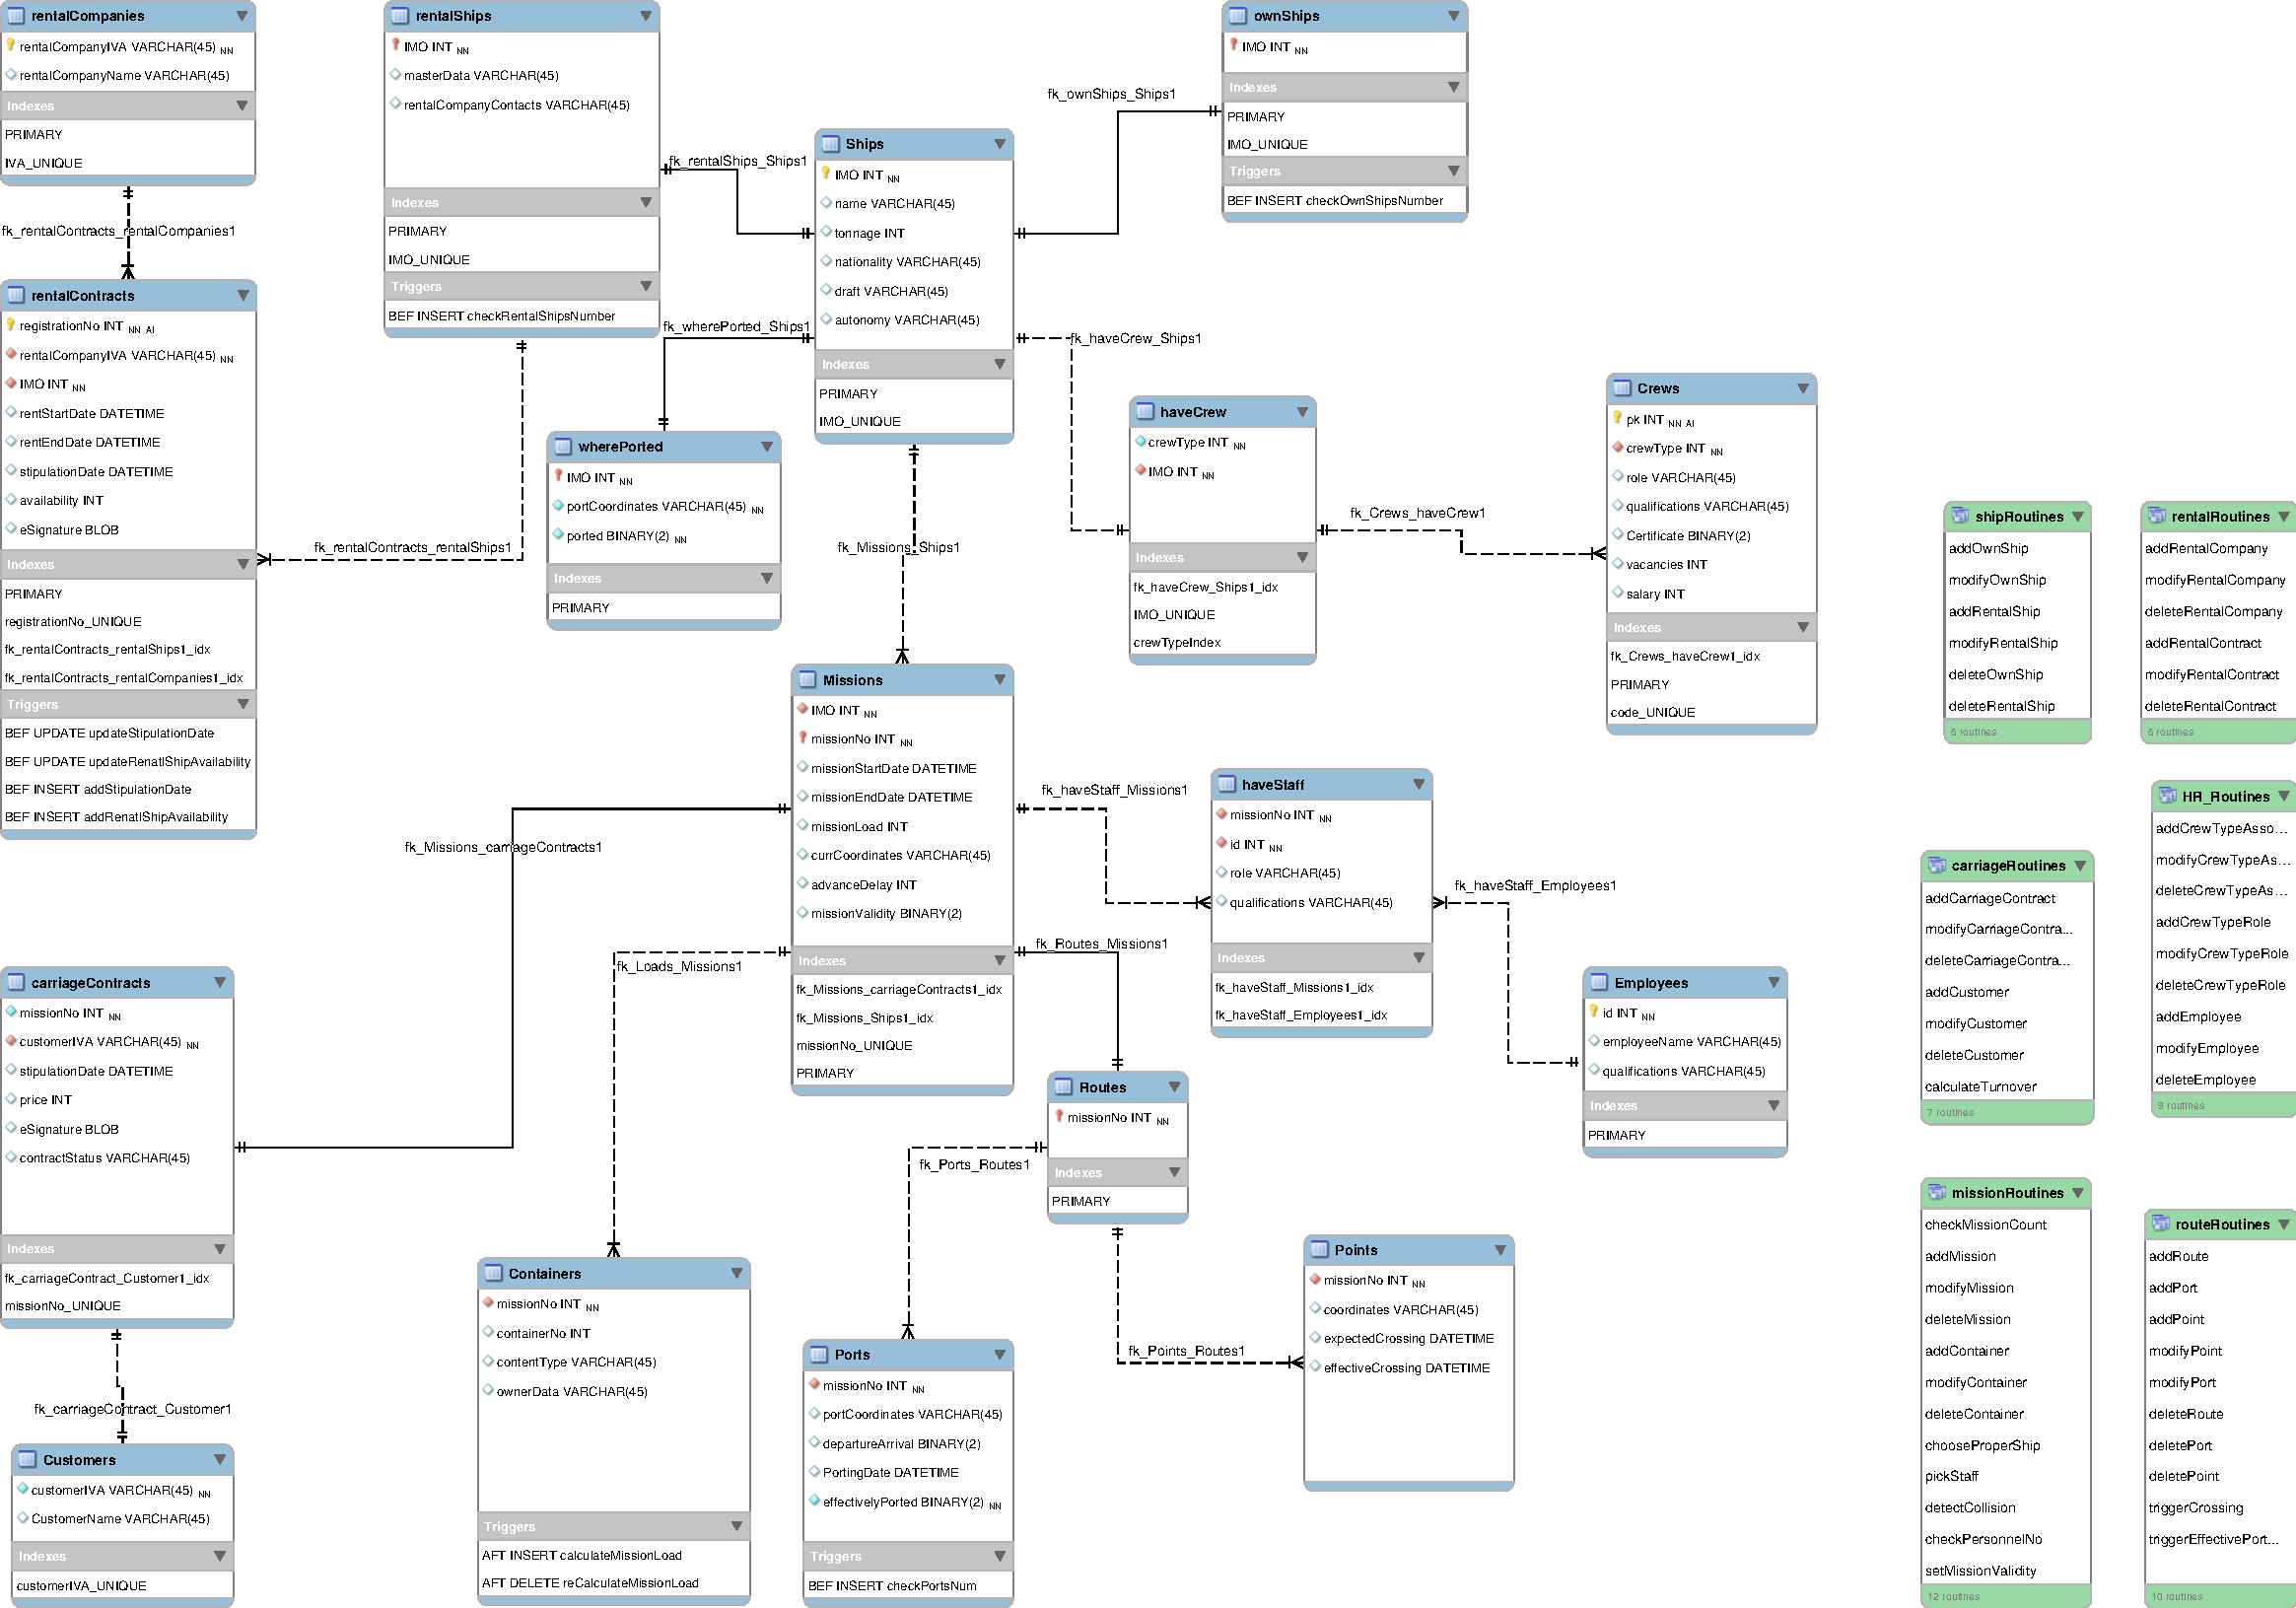
\includepdf[pagecommand={\section*{Conceputal Schema} \thispagestyle{empty}}]{MercantileShips-EER.pdf}
\newpage
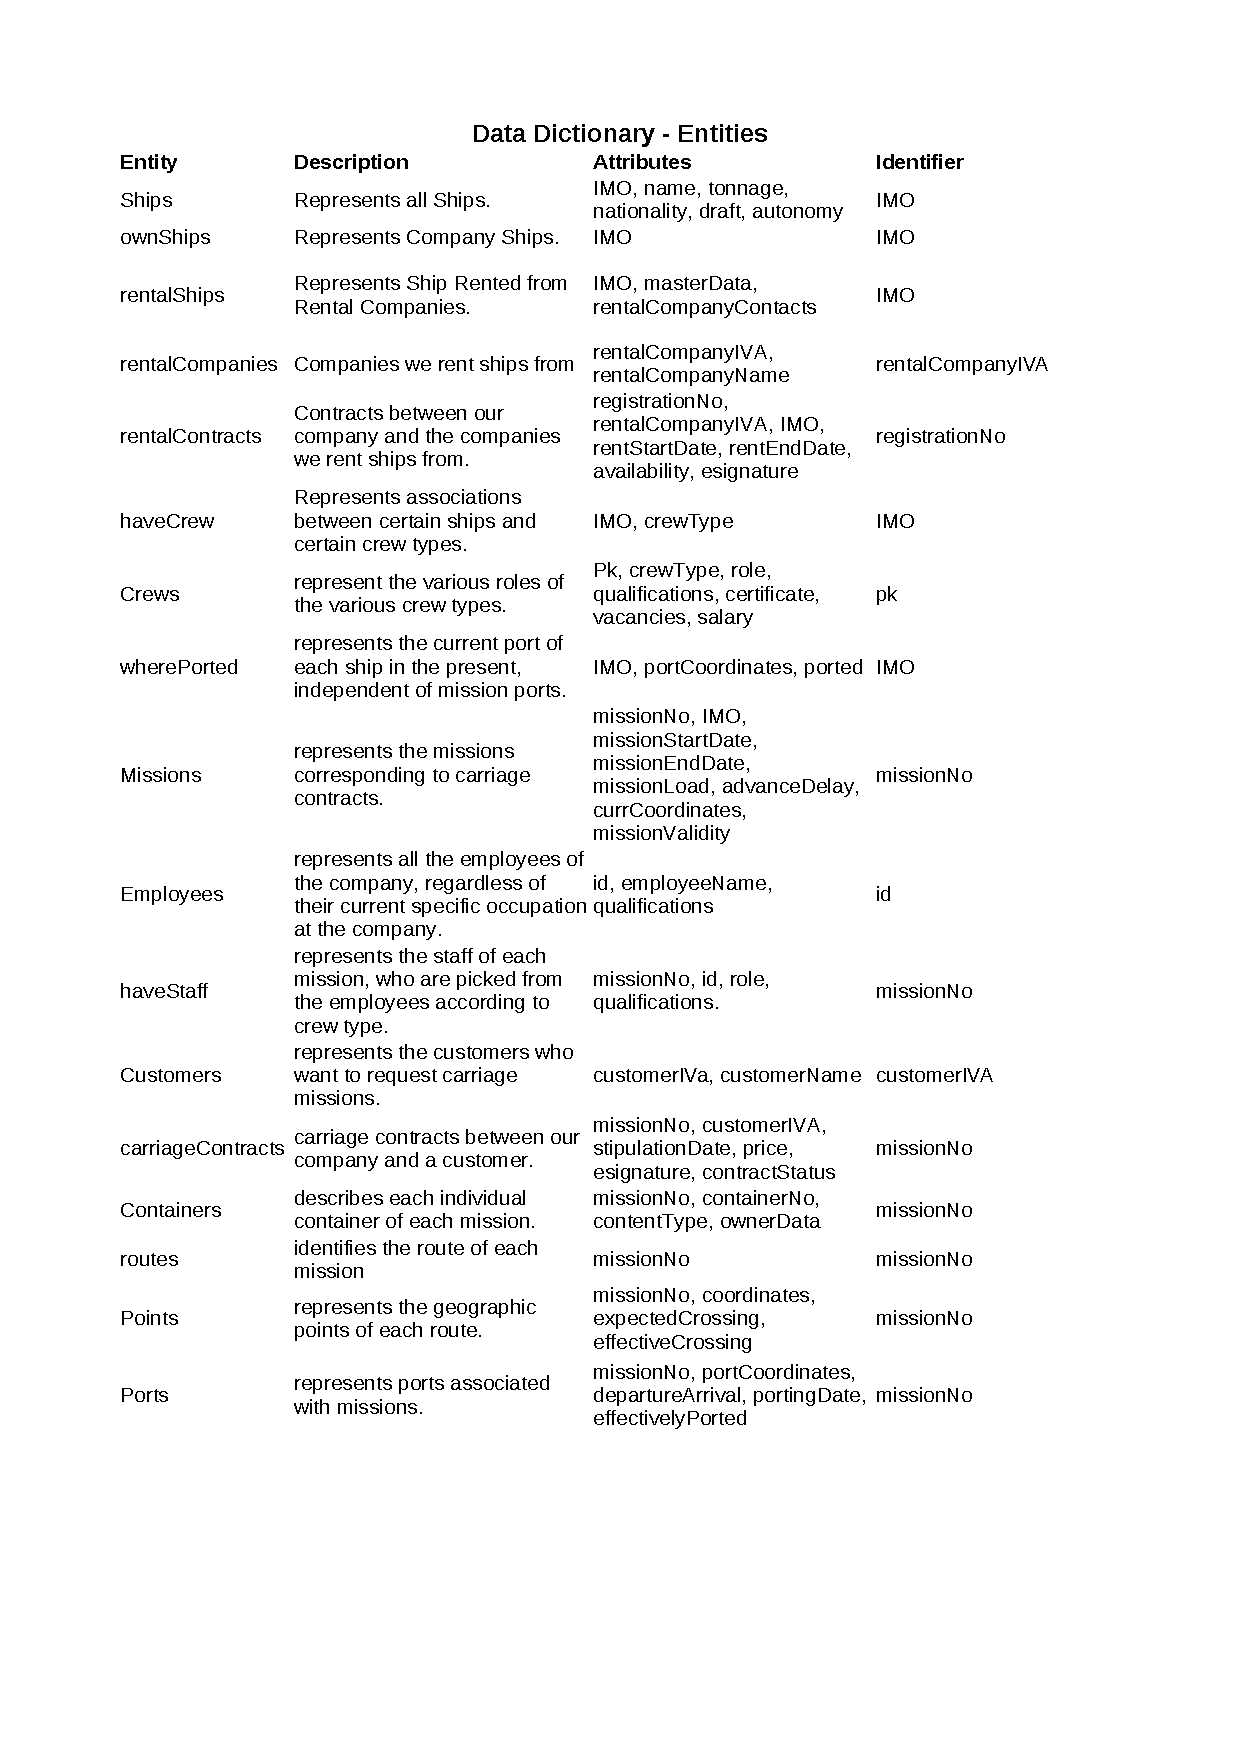
\includepdf[pagecommand={\thispagestyle{empty}}]{DataDictionary1.pdf}

\begin{flushleft}
	\section*{\textbf{Code Repository}}
\end{flushleft}
\begin{flushleft}
	A Github repository exists for this project under:\\
\end{flushleft}
	\begin{center}
		\url{https://github.com/AlyShmahell/Navibus-Mercatoriis}
	\end{center}
	
\end{document}
